%%
%% 研究報告用スイッチ
%% [techrep]
%%
%% 欧文表記無しのスイッチ(etitle,jkeyword,eabstract,ekeywordは任意)
%% [noauthor]
%%

\documentclass[submit,techrep]{ipsj}
%\documentclass[submit,techrep,noauthor]{ipsj}



\usepackage[dvips]{graphicx}
\usepackage{latexsym}
\usepackage{multirow}
\def\Underline{\setbox0\hbox\bgroup\let\\\endUnderline}
\def\endUnderline{\vphantom{y}\egroup\smash{\underline{\box0}}\\}
\def\|{\verb|}

\setcounter{巻数}{53}%vol53=2012
\setcounter{号数}{10}
\setcounter{page}{1}


\begin{document}


\title{個人情報及び個人識別子を含むファイルと通信を\\
検出するための双子の環境}


\affiliate{tsukuba}{筑波大学\\
University of Tsukuba}


\author{張 世申}{Zhang Shishen}{tsukuba}
\author{新城 靖}{Yasushi Shinjo}{tsukuba}
\author{三村 賢次郎}{Kenjiro Mimura}{tsukuba}


\begin{abstract}
インターネットユーザは普段ネットワークサービスを利用する時に,意図せず個人情報や個人を識別できる情報をサービス提供者に送信することがある.ユーザのプライバシを保護するために,ファイルやネットワーク通信からそのような情報を検出し除去したいが,現在のアプリケーションは複雑であり,それは容易なことではない.そのため本研究ではコンテナ技術を利用し,双子の環境という仮想実行環境を提案する.双子の環境とは,プログラムファイルやデータファイル等の内容がほとんど同じであるような2つの仮想実行環境である.双子の環境を利用する双子のブラウザを実装する.
\end{abstract}


\begin{jkeyword}
ユーザトラッキング,HTTP,コンテナ,ブラウザ
\end{jkeyword}



\maketitle


\section{はじめに}
PCで動作するアプリケーションは,Webブラウザのように明示的に通信を行うものだけでなく,オフィスツールのように,ユーザの意図しない通信を行うものがある.Webブラウザであっても,ユーザトラッキングのために暗黙的に通信を行うことがある.このような意図しない通信により住所・氏名等の個人情報,およびcookieのように個人情報と結び付けられた個人識別子が送信されることがある.

本研究では,コンテナというOS層の仮想実行環境を利用し,個人情報及び個人識別子が含まれているファイルと通信を検出することを提案する.そして,ファイルや通信から不要な情報を削除するツールを実装する.個人情報および個人識別子を検出する対象は,次の2つである.
\begin{itemize}
\item
ファイル
\item
ネットワーク通信 
\end{itemize}

たとえば,Webブラウザは,個人識別子として訪問履歴や,フォームの内容,Cookieなどを保存する.ユーザトラッキングでよく利用されるCookieにはサーバが配るユニークなIDやセッションIDが含まれている.しかし,現在のWebブラウザやオフィスツールは,非常に複雑であり,これらの識別子がどのファイルにどのような形式で保存されているかを調べることは容易ではない.本研究では,双子の環境を実装して,個人情報および個人識別子が含まれているファイルや通信を検出する.なお,以下では,個人情報と記載した時にも,個人情報と個人識別子の両方を含むものとする.


\section{双子の環境と双子のブラウザによる個人情報の検出}
\label{twinsBrowser}
双子の環境とは,プログラムファイルやデータファイル等の内容がほとんど同じであるような2つの仮想実行環境である(図1).人間における双子の研究では,異なる双子が異なる環境で育てられた際にそれぞれの医学的,遺伝子的,心理学的性格を調査ことで,どのような違いが生まれるかを調査する場合が多い.本研究で提案する双子の環境では,類似の2つの環境で同一のプログラムをそれぞれ実行し,同一の入力を与える.そして,2つのプログラムの動作上の相違点を検出する.

\begin{figure}[t]
\begin{center}
\includegraphics[width=8cm]{img/first.eps}
\caption{双子の環境}
\label{figure:twin}
\end{center}
\end{figure}



本研究では,双子の環境で動作するWebブラウザとして,双子のブラウザを開発している\cite{comsys}.双子のブラウザとは,双子の環境で協調動作する2つのブラウザである.

本研究では,双子のブラウザを用いてサーバによるユーザトラッキングを検出する.ユーザトラッキングの手法としては,Cookieを使う方法やURLにタグを埋め込む方法がある.それ以外に,Flash CookieやHTML5のIndexedDBなどのストレージを使う方法もある.本研究では双子のブラウザを用いてブラウザが作成する全てのファイルの差分およびブラウザが発信するネットワーク通信の内容の差分を調査する.その差分にユーザトラッキングのための情報が含まれる可能性が高い.その差分を削除,または修正することでユーザトラッキングを阻止することができると思われる.




\subsection{コンテナによる双子の環境の実装}
本研究では,環境内のファイルを調査するが,一般的な仮想マシンではホストはゲスト OS のファイルシステムを直接的アクセスできないという問題がある.そこで本研究では,コンテナという OS 層の仮想マシンを使う.

コンテナは,仮想化技術の一種である.VMwareやXen,KVMなとの一般的な仮想マシンとは違い,コンテナはハードウェア層ではなく,OS層の仮想マシンである.コンテナはLinuxカーネルのcgroupsとnamespaces機能を利用し,リソース管理と隔離を提供している.


本研究ではコンテナを実装する仕組みとして Dockerを使う. Dockerでは, Overlay File System というファイルシステムが利用可能である.このファイルシステムではゲストOSのファイルをホストOSからアクセスできるため,ファイルの差分を取得することが容易である.

ゲストOSが生成したファイルはOverlay File SystemのUpper Layerに保存される.したがって,Upper directoryのみ読み込むことでファイル内容の変化を得ることができる.




\begin{figure*}[ht]
\begin{center}
\includegraphics[width=16cm]{img/file.eps}
\caption{Docker Overlay Filesystemによるファイル差分検出}
\label{figure:file}
\end{center}
\end{figure*}

\begin{figure*}[ht]
\begin{center}
\includegraphics[width=16cm]{img/net.eps}
\caption{MITM-proxyを用いたHTTPのメッセージの差分検出}
\label{figure:network}
\end{center}
\end{figure*}


\subsection{ファイルの差分検出}
\label{cha:file}

図\ref{figure:file}に,ファイルの差分検出の仕組みを示す.まず,同じイメージを利用する2つのコンテナを起動し,対象となるプログラム(主に双子のブラウザ)を実行する,ホストからの入力を2つ複製して,2つのコンテナを操作する.それからコンテナが生成したファイルをホストOSで取得する.そして,ファイルの種類ごとにファイル内容に前処理を行い,その結果をdiffコマンドに与える.

\label{sec:prep}
プログラムでよく利用される保存形式としてはテキスト形式,データベース形式,および,マーシャリング形式の3つがある.マーシャリング形式としてはよくJSONとXMLがよく使われる.本研究ではWebブラウザFirefoxとGoogle Chromeのファイル保存形式を調査した.その結果,テキスト,JavaScript,JSON,XML,SQLite,BerkeleyDB,LevelDBの7種類あることがわかった.

コンテナが出力するファイルがテキストファイルであれば,そのままdiffコマンドで差分を取ることができる.しかしながら,JSONやXMLでは,そのままdiffコマンドに与えても大量の出力がなされ,目的とする個人情報が埋もれてしまうという問題がある.また,diffコマンドは,バイナリファイルを扱うことができない.

そこで本研究ではプログラムが生成したファイルに対して前処理を行い,diffで差分を取る前に識別しやすい形に変換する(図\ref{figure:file}).形式分類モジュールで,ファイルを形式で分類する.

分類した後、形式ごとにテキスト化する。主な形式について、テキスト化の方法を以下に示す。
\begin{itemize}
\item
SQLiteデータベース。
まず、sqlite3のdumpサブコマンドでテキストに変換する。次に、自動増加の主キー列を削除する。
\item

\subsection{タイムスタンプの扱い}
\label{cha:timestamp}
ネットワーク通信を行うプログラムは,様々なタイムスタンプをファイルに保存する.単純にファイルの差分を得ると,タイムスタンプの差によるものが大量に生成され,重要な差分が埋もれてしまう.

本研究では,タイムスタンプを次のように分類して扱う.


\begin{description}
\item{・リモート: }
リモートの通信相手が指定したもの.例えば,HTTPの``Last-Modified:"ヘッダに由来するもの.
\item{・ローカル: }
ローカルのOSからシステム・コールで取得したものに由来するもの.
\end{description}


リモート・タイムスタンプは,外部に発信されることが想定されている.例えば,HTTPの応答メッセージに含まれた``Last-Modified:"ヘッダの値は,同じコンテンツを再取得する時に,要求メッセージの``if-Modified-Since:"ヘッダに含まれて発信される.この値は,個人識別子としてユーザトラッキングに使われることがあることが知られている.

一方,ローカル・タイムスタンプは,外部に発信されなければ,個人識別子にはなり得ない.したがって,双子の環境の実装では,ローカル・タイムスタンプの違いを排除したい.本研究では,双子の環境で実行したタイム関連のシステム・コールgettimeofday()とclock\_gettime()をオーバーライドする.そのため,本研究で作成した動的リンクライブラリをLD\_PRELOADで置き換える.置き換えたシステム・コールは,環境変数で指定された固定の日付を返す.


このような処理を行ったとしても,アプリケーションの内部で独自にシステム・コールで得たタイムスタンプを加工して利用していることがある.例えば,Firefoxでは,システム・コールclock\_gettime()で得られたナノ秒単位の時刻に,1から4まで加えた値を利用している.この問題を解決するために,本研究では,テキスト化した後,ローカル・タイムスタンプとそれを加工したものと思われる数字を定数で置き換える.

\subsection{ランダム性の排除}

プログラムは多く予想出来ない行動を行う.その結果,ファイルの内容に差が生まれ,本来検出したい個人情報を覆い隠してしまう.そこで,本研究では,そのようなランダムな行動を排除する.

まず,乱数によるプログラムのランダム行動を抑止するために,乱数デバイス/dev/urandomを置き換える.本研究では擬似乱数生成器デバイスドライバを作り,双子のコンテナのインスタンスに同じシードを与える.

マルチスレッドやマルチプロセスのアプリケーションのスケジュールも実行結果に影響を与える.ChromeブラウザのTaskモデルは,UIとIOスレッド以外にワーカスレッドが多数存在する.一つの作業がどのワーカスレッドにより実行されるか予想できない.その結果,Chromeブラウザでの実験中には,TIDのような予測できない結果が出力される.そして,PCのリアルタイムパフォーマンスによる動的にワーカスレッドの数を調整することもある\cite{dynamic}.そこで本研究では,テキスト化してダンプする時にスレッド識別子を含まないようにする.

\subsection{ネットワークメッセージの差分}
\label{sec:net}

コンテナが生成したファイルだけではなく,ネットワーク通信の内容に個人識別情報も多く存在する.これらのメッセージも差分を取って個人情報を検出したい.本研究ではブラウザアプリケーションを使って,ブラウザ通信を対象としてネットワークメッセージをキャプチャする.以前のWebブラウザとHTMLのバージョンは,HTTP Request-Responseに基づくだけが,多数のシナリオには効率が低いから,新しいHTML5には多くの新しいプロトコルを提出した.また,既存のRequest-Responseの形のHTTPプロトコル(HTTP1.1)もいろんな制限があるし,今はHTTP2.0が提出され,多くの場合で使用される.それ以外にコンテナ内で実行されるプログラムが送受信されているメッセージは,HTTPSにより暗号化されてることがある.そこで,本研究では,MITM-Proxy(Man-In-The-Middle-Proxy)\footnote{https://mitmproxy.org/}を使ってHTTPやHTTPSの通信をキャプチャする.

\subsubsection{Man-In-The-Middle Proxyによるネットワーク通信のキャプチャ}

MTIM-Proxyは,対話型のHTTPSプロキシであり,Python APIを利用する簡単でHTTPとHTTPSの通信をキャプチャ,修正することができる.一般的な通信プロキシの機能の上で,いくつのHTML5機能も加え,Keep-Aliveなどの持続的接続機能もつける.MITM-Proxyは以下の通信プロキシをよく支持する.
\begin{itemize}
\item
Raw通信
MITM-ProxyにはTCP通信のキャプチャとフィルタを実装した.
\item
HTTPとHTTPSの通信
HTTPSの通信のキャプチャはTLS層を全部transparent-proxyの形式でフィルタし,ユーザはHTTP通信だけ見える.
\item
websocketの通信
HTML5の新しいプロトコルとしてよく使われる.HTTPメッセージとは違い,双方向の通信である.MITM-Proxyにはwebsocket通信を支持し,Connectionと通信のキャプチャができる.

\end{itemize}

他の通信型もいくつある.例えばメディア通信でよく使われたWebRTC(Web Real-Time Communications)プロトコル,FlashやSilverlightなどのプラグインによる通信.これらの通信のキャプチャはまだ実装してない.

\subsubsection{通信データのテキスト化とDump}

ネットワーク通信の差分取る仕組みを図\ref{figure:network}に示す.HTTP通信の内容をKey-Valueの形式に変える.Keyとしては現在RequestのURLをQuery Stringを排除した部分と訪問の回数を用いている.Valueは残りのQuery String, Header, body, Response Header, bodyにする.Dumpした内容はHTTP通信のヘッダContent-TypeやContent-Encodingによる分類して,ふさわしい処理を行う.例えば"Content-Encoding: gzip"ヘッダの通信は圧縮した形を展開し,"Transfer-Encoding: chunked"ヘッダの通信はchunkの属性のよって,多数のChunkを組み合わせる.それから,全部のテキストファイル,例えばhtmlやjavascript,cssなどのファイルはテキストファイルとして\ref{sec:prep}節で述べたファイル差分検出モジュールに与える.テキストファイルではない通信,例えばpng,faviconなどの通信はバイナリファイルとして扱う.Websocketの通信はFull Duplexであるから,一つのURLが多数の通信を行う.WebsocketのKeyはURLと通信の回数,送受信方を用い,Valueは通信の内容にする.

\section{双子のブラウザの実装}
本研究では,個人情報と個人識別し以外の差分を最低限にするために2つのブラウザを同時に動かす.
この双子のブラウザは,図\ref{twin-brow}のように親ブラウザがあり,このブラウザを実際に操作し同じ操作を2つの子ブラウザに与える.


双子のブラウザは,大きく親ブラウザの操作を読み取る部分と子ブラウザを操作する部分に分けられる.
ブラウザの操作を読み取る部分は,WebExtensions\footnote{WebExtensions: https://developer.mozilla.org/ja/Add-ons/WebExtensions}を用いてブラウザの機能を拡張することで実現する.
このWebExtensionsは,Google ChromeとFireFoxでほぼ同じように動作する.
発生した操作を検知するために,親ブラウザが表示するWebページのDOMに対して予めイベントを登録しておく.
イベントが発生した場合には,発生したイベント名(クリックや入力など)と対象のDOMを送信するように登録しておく.
対象のDOMの記述には,Xpathを用いる.また,イベントがどのタブで発生したか判別できるようにタブIDも同時に送信する.

ブラウザを操作する部分は,Selenium\footnote{Selenium: http://www.seleniumhq.org/}を用いて実装する.
Seleniumは,Webブラウザの自動化用ツールであり,JavaやPython, Node.jsからWebブラウザのマウスやキーボードを使った操作を入力する.
子ブラウザは,親ブラウザで発生したイベントの種類に応じて,Seleniumライブラリを介して操作する.
子ブラウザには,初めウィンドウが存在しないためSelniumによってタブを作成し,要求されたURLを表示する.
この時,タブのハンドラと送られてきた親ブラウザのタブIDの対応を保持しておく.
すでに親ブラウザで開かれたタブは,子ブラウザの対応するタブに操作をすることで,
親と子ブラウザで複数のタブを協調する.

双子のブラウザの実装を図\ref{cobrow}に示す.
この環境で同じ動作を行えるものを以下に示す.
\begin{itemize}
\item { クリック}
\item{ フォームのinput要素の入力 }
\item{ スクロール}
\item{ウィンドウのリサイズ}
\end{itemize}	

\begin{figure}[t]
\begin{center}
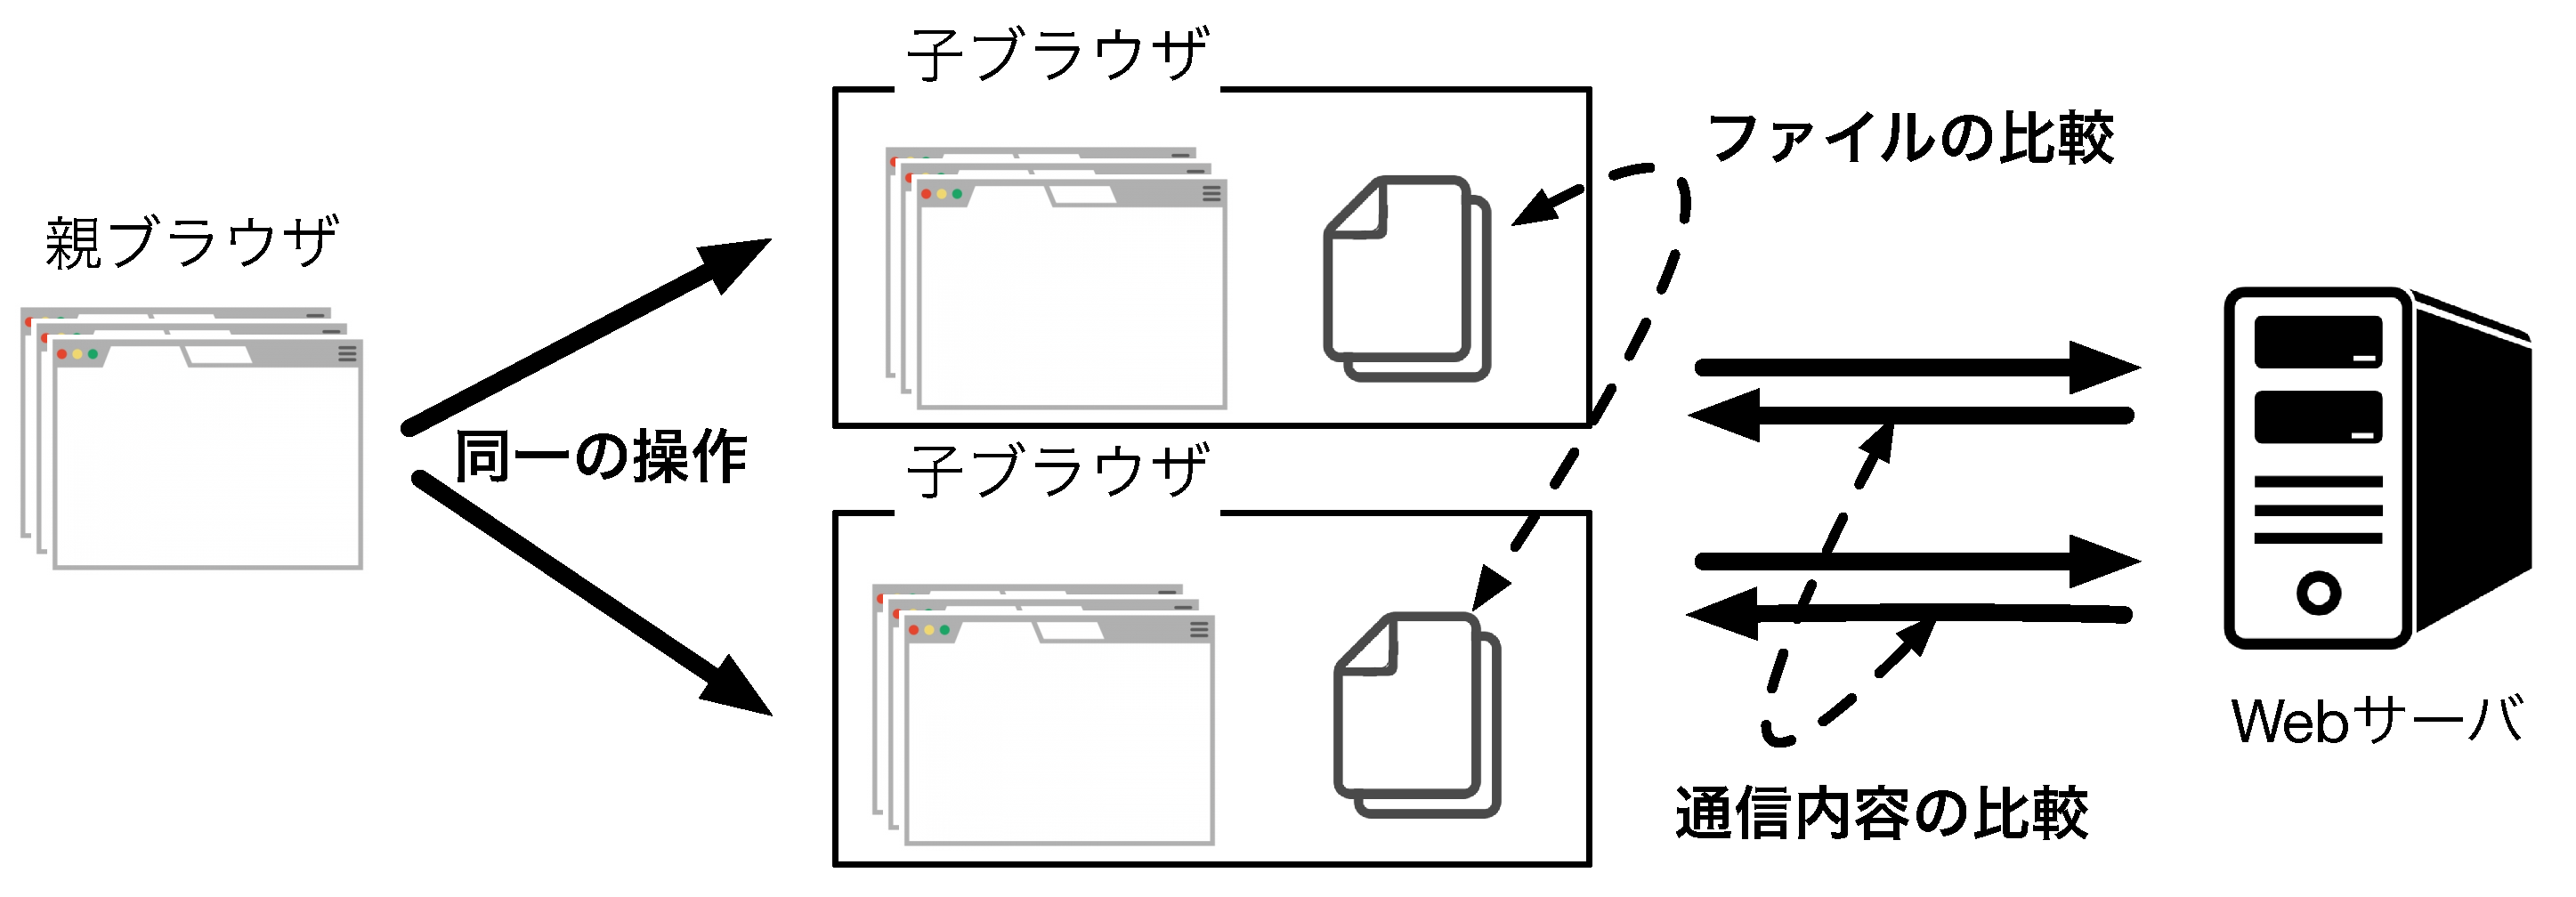
\includegraphics[width=8cm]{img/twin-brow-p.eps}
 \caption{双子のブラウザ}
  \label{twin-brow}
  \end{center}
\end{figure}

\begin{figure}[t]
\begin{center}
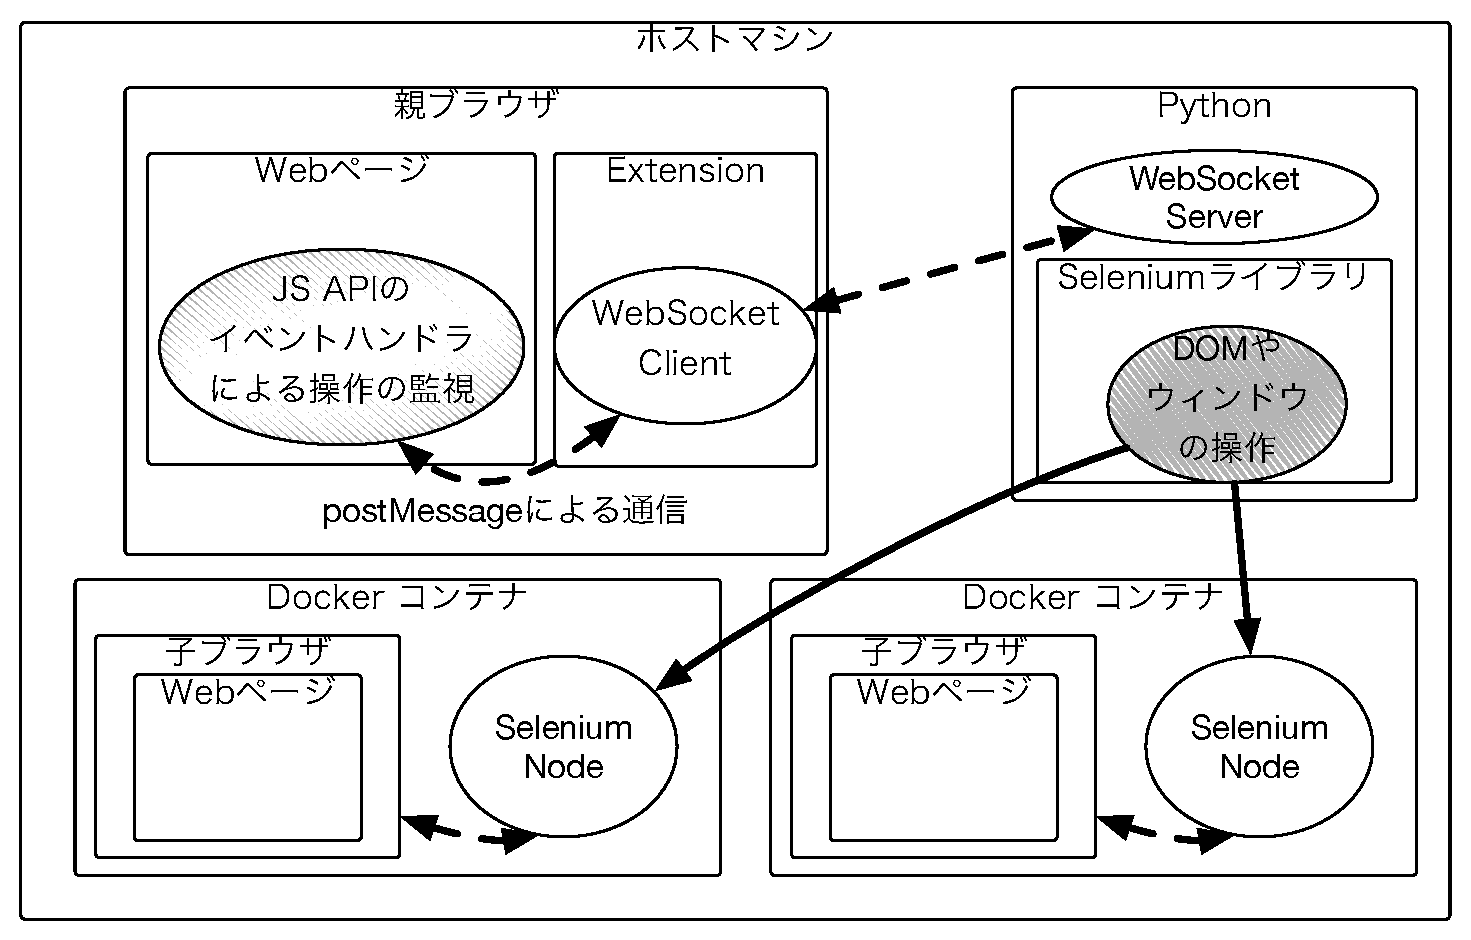
\includegraphics[width=8cm]{img/cobrow-3.eps}
 \caption{Seleniumによる双子のブラウザの実装}
  \label{cobrow}
  \end{center}
\end{figure}


\begin{table*}[ht]
\caption{差分がないファイルと差分があるファイルの数}
\centering
\begin{tabular}{|p{2cm}|l|p{1.9cm}|p{1.9cm}|l|p{1.9cm}|p{1.9cm}|}
\hline
&\multicolumn{3}{|c|}{\footnotesize{Firefox}}&\multicolumn{3}{c|}{\footnotesize{Google Chrome}}\\
\hline
&\multirow{2}{1.5cm}{\footnotesize{個人情報がない}} &
\multicolumn{2}{c|}{\footnotesize{差分がある}} &\multirow{2}{1.5cm}{\footnotesize{個人情報がない}}&
\multicolumn{2}{c|}{\footnotesize{差分がある}} \\
\cline{3-4}\cline{6-7}
  & & \footnotesize{不明なバイナリ} & \footnotesize{テキストと扱えるバイナリ(行数)}& &\footnotesize{不明なバイナリ} & \footnotesize{テキストと扱えるバイナリ(行数)} \\
\hline
\footnotesize{更新されたファイル}&\multicolumn{1}{r|}{\footnotesize{52}}&\multicolumn{1}{r|}{\footnotesize{0}}&\multicolumn{1}{r|}{\footnotesize{7(28)}}  & \multicolumn{1}{r|}{\footnotesize{98}} & \multicolumn{1}{r|}{\footnotesize{5}} & \multicolumn{1}{r|}{\footnotesize{47(114)}} \\
\hline
\footnotesize{乱数生成器の置き換え}&\multicolumn{1}{r|}{\footnotesize{55}}&\multicolumn{1}{r|}{\footnotesize{0}}&\multicolumn{1}{r|}{\footnotesize{4(10)} }& \multicolumn{1}{r|}{\footnotesize{128} }& \multicolumn{1}{r|}{\footnotesize{5} }& \multicolumn{1}{r|}{\footnotesize{17(46)}} \\
\hline
\footnotesize{ローカルタイムスタンプの固定}&\multicolumn{1}{r|}{\footnotesize{55}}&\multicolumn{1}{r|}{\footnotesize{0}}&\multicolumn{1}{r|}{\footnotesize{4(8)} }&  \multicolumn{1}{r|}{\footnotesize{128} }& \multicolumn{1}{r|}{\footnotesize{5} }&\multicolumn{1}{r|}{\footnotesize{17(41) }}\\
\hline
\footnotesize{前処理後}&\multicolumn{1}{r|}{\footnotesize{55}}&\multicolumn{1}{r|}{\footnotesize{0}}&\multicolumn{1}{r|}{\footnotesize{4(8)}} &\multicolumn{1}{r|}{ \footnotesize{136} }& \multicolumn{1}{r|}{\footnotesize{5} }&\multicolumn{1}{r|}{\footnotesize{9(15)}}\\
\hline
\end{tabular}
\label{fig:result}
\end{table*}

\begin{table*}[ht]



\caption{ファイルの差分の例}
\centering

\begin{tabular}{ |l|p{6cm}|p{6cm}| }

 \hline
 \footnotesize{ファイル名} &\footnotesize{コンテナ1} &\footnotesize{コンテナ2}\\
 \hline
 \footnotesize{cookies.sqlite} & \footnotesize{value = 132=S1fjWe4xjUJJowuImYQyi...} & \footnotesize{value = 132=ablTT1GOqBlYlBX-MQ...}\\
\hline
 \footnotesize{places.sqlite} & \footnotesize{guid = xhIxtPu6zAJ7} & \footnotesize{guid = IlfETnEs0Dr4}\\
\hline
 \footnotesize{sessionstore.js} & \footnotesize{"docshellUUID": "\{4c4508da-9468-430b-8eac- 0484dcc43e5d\}"} & \footnotesize{"docshellUUID": "\{bfcff6ba-42c2-4731-a65c- ae1ba7b1cc0e\}"}\\
 \hline
\footnotesize{prefs.js} & \footnotesize{user\_pref("browser.slowStartup.averageTime", 14971)} & \footnotesize{user\_pref("browser.slowStartup.averageTime", 18103)}\\
\hline
\end{tabular}
\label{fig:data}
\end{table*}



\section{個人識別情報の削除}

\ref{twinsBrowser}章で述べた方法で個人識別情報を含むファイルとネットワーク通信を検出した後,本研究では,それを削除するツールを実装する.

\subsection{ファイルから個人識別情報の削除}

現在のWebブラウザやオフィスツールは,非常に複雑であり,多くのファイルをアクセスする.個人識別情報は,これらのファイルのうち,更新されるものに保存される.本研究では,\ref{}節の手法により,更新されるファイルを特定することができる.これらの更新されるファイルを削除すれば,個人識別情報も削除されるが利便性が大きく低下することがある.たとえば,Webブラウザでは,ブックマークや個人の設定を保存するファイルが更新されるが,それらを全て削除すると,利便性が低下する.

そこで本研究では,更新されるファイルを,次の3種類に分類する.
\begin{itemize}
\item
アプリケーション自身が個人識別情報を削除する機能を提供しているもの.たとえば,Webブラウザなら,cookieを終了時に削除する機能がある.
\item
ファイル全体を削除すると問題が生じるもの.
\item
ファイル全体を削除しても問題が生じないもの.
\end{itemize}

本研究では,ファイル全体を削除すると問題が生じるものについて,内部の個人識別情報を特定し,削除するか,ランダムな値で置き換えるツールを作成する.

本研究では,Webブラウザの次のファイルから個人識別情報を削除するツールを作成する.

\begin{itemize}
\item
Firefox cookies.sqlite
persistant cookieのvalueをランダムな値で置き換える.
\item
Firefox pref.js
時刻に関する行(browser.slowStartup.averageTime等)を削除する.

\item
Firefox places.sqlite
guidをランダムな値で置き換える.
\item
Firefox sessionstore.js
docshellUUIDをランダムな値で置き換える.
principalToInherit\_base64をランダムな値で置き換える.
\end{itemize}

本研究では,Webブラウザの次のファイルを削除とタグの書き換えをしても問題が生じないことを確認した.

\begin{itemize}
\item
Firefox cookies.sqlite
ファイルを直接に削除とpersistant cookieのvalueをランダムな値で置き換える両方とも問題がない.ただし,valueを書き換えてもう一度ブラウザをオープンしサイトを訪問すると,値が更新された.
\item
Firefox pref.js
ファイルを削除するとブラウザは普通に作動するが,consoleからWARNINGがいくつ出る
時刻に関する行(browser.slowStartup.averageTime等)を削除すると問題がない

\item
Firefox places.sqlite
ファイルを削除とguidをランダムな値で置き換えるには問題がない.ただし,guidをランダムな値で置き換えて,もう一度ブラウザをオープンしサイトを訪問すると,値が更新されてない.
\item
Firefox sessionstore.js
docshellUUIDをランダムな値で置き換えるとprincipalToInherit\_base64をランダムな値で置き換えるには問題がない

\end{itemize}



\subsection{ネットワーク通信から個人識別情報の削除}

ファイルからの個人識別情報の削除は,プログラムを一度終了しなければ行うことができない.たとえば,WebブラウザFirefoxのplaces.sqliteに含まれるguidは,本研究のツールで削除できる.しかし,ブラウザの実行中には,このツールは動作しない.

アプリケーション自身が,個人識別情報の送信を抑止する機能を持っていることがある.たとえば,Webブラウザは,cookieを送信しない機能や,検索結果のURLから個人識別情報を削除する拡張機能を持っている.Webブラウザについては,このような既存の機能を利用すれば,かなりの個人識別情報を削除することができる.しかしながら,Webブラウザの機能には,ユーザがアクセスするページではないネットワーク通信を扱えないという限界がある.たとえば,WebブラウザがSSL/TLSの証明書を検証するためにOnline Certificate Status Protocol(OCSP)に基づき行う通信を扱えない.また,Webブラウザ以外のアプリケーションについては,ネットワーク通信から個人識別情報を削除する機能は開発されていない.本研究では,MITM-Proxyを用いてネットワーク通信から個人識別情報を削除する.具体的には,次のようなメッセージから個人識別情報の削除する.
\begin{itemize}

\item
ファイルシステムに検出した個人識別情報

個人情報はネットワークアプリケーションにより,ファイルに保存したデータを悪意のあるサーバに送信することがある.この状況を防ぐため,ファイルで検出した個人識別情報はネットワーク通信の内容と比較して,同じである部分をネットワーク通信内容から削除する必要がある.


\item
サーバから送信した情報

cookieなどの個人情報は,まずHTTP通信よりサーバからクライアントに送信する.この原因でサーバからのメッセージを通信中に検出し,ファイルと同じようにdiffで差分を取った部分は,個人識別情報である可能性が高い.これらの差分情報を記録して,クライアントが送信したメッセージをフィルタする.

たとえばHTTP Responseのヘッダには``Set-cookie:"行があった時に,クライアント端に個人識別子になるcookieが保存される.しかし全部のcookieがユーザトラッキングに使われるではなく,ログインやショッピング用に使われたsessionのストアと,ユーザのセッティングに使われる場合もある.これらのcookieを削除するとブラウザの使用には問題が生じるかもしれない.そこで本研究は,サーバのresponseについたcookieのexpiryを検出,長期間保存したcookieを記録し,クライアントのresponseの中に記録したcookieが含まれた時にHTTPヘッダのcookieラインを削除する.

\end{itemize}

個人情報の検出と通信中の内容削除は,HTTP RequestとHTTP Responseの形で実行する.HTTP通信の中に,もっとも重要な部分はHTTPヘッダである.ヘッダには多くの通信のメタデータが含む.

Webサーバは,IPアドレスやブラウザのフィンガープリント等のメタ情報を使ってユーザトラッキングを行うこともある.送信するメッセージの内容だけを操作しても,それには限界がある.本研究では,IPアドレルを隠すことについては,Tor等の既存の手法と組み合わせて用いることにする.








\begin{table*}[ht]
\caption{ネットワーク通信の差分の数}
\centering

\begin{tabular}{ |p{5cm}|p{5cm}| }

 \hline
 全部の通信数 &\footnotesize{21}\\
 \hline
  \footnotesize{差分がある通信} & \footnotesize{20}\\
\hline

  \footnotesize{応答に差分がある数} & \footnotesize{2}\\
 \hline
\footnotesize{タイムスタンプと重複を排除の差分} & \footnotesize{22(行)}\\
\hline
\end{tabular}
\label{fig:netdiff}
\end{table*}


 
 


\begin{table*}[ht]
\caption{ネットワーク通信の差分の例}
\centering

\begin{tabular}{ |p{3.5cm}|p{5cm}|p{5cm}| }

 \hline
 URL &コンテナ1 &\footnotesize{コンテナ2}\\
 \hline
 \footnotesize{www.google.com} & \footnotesize{Cookie:1P\_JAR=2017-12-12-04,NID=119=BGA6eL4YT9Q...} & \footnotesize{Cookie:1P\_JAR=2017-12-12-04,NID=rzmrga\_L3s...}\\
\hline
 \footnotesize{www.google.com/gen\_204} & \footnotesize{ei:pdcsW5TSLIb28AXosLGYBA} & \footnotesize{ei:pdcsW-vCDMfS8QWq-I34Bg}\\
\hline
 \footnotesize{ssl.gstatic.com/gb/ima ges/i1\_1967ca6a.png} & \footnotesize{age:253629} & \footnotesize{age:253628}\\
 \hline

\end{tabular}
\label{fig:data}
\end{table*}






\section{実験}
\subsection{双子のブラウザが生成したファイルの差分}
\label{sec:file}

本研究室ではFirefoxとGoogle Chromeで双子のブラウザを実装している.今回,ユーザトラッキングを行っている代表的なWebサイトとしてGoogleを選択しhttp://www.google.com/を訪問する実験を行った.これは,ログインを必要としない簡単なサイトである.

\subsubsection{Firefox}
まずFirefoxブラウザを双子のブラウザとして双子の環境で実行した.コンテナの全てのファイルの変化をリストアップしたところ,全部で59個のファイルが作成された.その中に29個が~/.cacheにある一時的なファイルのためファイル名によるフィルタにより自動的に除外された.残る30個のファイルに対して前処理を行って,テキスト化しdiffコマンドで差分を取った結果は全部28行であった.\ref{cha:file}章で述べた方法に従ってテキスト化した差分を削減した結果,最終的に差分は8行だった.識別できないバイナリファイルはなかった.

表\ref{fig:data}に,発見した差分の一部を示す.cookies.sqliteには,HTTP Cookiesが保存されていることがわかる.places.sqliteは,訪問履歴を保持するファイルである.その中に,アクセスしたURLが保存されている.このように,URLの中に,ユーザトラッキングに利用可能なタグが埋め込まれていることがわかる.

この実験の結果,提案手法により,ファイルを特定し,使用者の識別子を検出することができ,ユーザトラッキングに使われる個人識別情報が含まれることが確認された.

\subsubsection{Chrome}

2番目の実験はGoogle Chromeで行った.結果を表\ref{fig:result}に表す.差分があるファイルはFirefoxより多い.識別できないバイナリファイルが5個残された.

\label{sec:one}
\subsection{ネットワーク通信内容の差分}
ブラウザが行うネットワーク通信の内容の差分を調査した.訪問したサイトは,\ref{sec:file}節と同じである.結果は\ref{fig:netdiff}に示す.

全部の通信の数は21個あり,テキスト形式のファイル以外にpngが6個,icoが1個あった.20個のメッセージの内容に差分があり,1番目の通信だけは差分がなかった.ネットワーク通信の差分はタイムスタンプと重複を除き全部で22行あった.応答メッセージの内容に差分があるファイルが2個あった.それらのURLはwww.google.comとwww.google.com/gen\_204であった.また,URLが違う通信の数は3個あった.

メッセージの内容にはcookiesが現れている.これは,cookies.sqlite(表\ref{fig:data})にも含まれている.




\section{関連研究}
Qubes-OS\cite{qubes}は高いセキュリティを実現するためのOSである.Qubes-OSは仮想計算機モニタ(Xen)を用いて,アプリケーションを隔離された仮想実行環境で実行する.Qubes-OSには,複数の仮想実行環境のファイルを比較する機能はない.

Blink-Docker\cite{blink}はコンテナ中でブラウザを実行することで,Canvas Fingerprintを利用したユーザトラッキングからユーザを保護する.Canvas Fingerprint はハードウェアや OS のわずかな違いによってクライアントを特定する手法である.Blink-Dockerはコンテナ技術を利用し,毎回 Fingerprint を変えることができる.本研究では,通信内容を検査し,そのようなユーザトラッキングを検出したいと考えている.



\section{まとめ}
本研究では人間の双子の研究に参考した双子の環境を提案した.本研究ではDockerコンテナを利用し,軽量で類似の仮想環境を作り,ファイルと通信内容に含まれる個人情報を検出する.

本研究室で開発された双子のブラウザを双子の環境で実行し,それらが生成するファイルの差分を調査するツールを実装した.また,Man-In-The-Middle Proxyを用いて,通信内容を比較するツールを実装した.実装した双子のブラウザを利用し,個人情報と個人識別子である可能性が高いユニークなタグがいくつ検出した.そして,個人識別子を変更の方で保護する.


%%%%%%%%%%%%%%%%%%%%%%%
%% ここまで本文
%%%%%%%%%%%%%%%%%%%%%%%


%%FIXME
%%bibファイルを指定する
\begin{thebibliography}{1}

\bibitem{qubes}
 {\small Qubes OS - A reasonably secure operating system: https://www.qubes-os.org/, accessed: 2017-11-22.}
\bibitem{blink}
 P Laperdrix, W Rudametkin, B Baudry: "Blink: A moving-target approach to fingerprint diversification" 37th IEEE Symposium on Security and Privacy, Poster Session, [Online]
http://www.ieee-security.org/TC/SP2016/poster-abstracts/59-poster\_abstract.pdf,  (2016).
\bibitem{dynamic}
Javier Verd, Juan Jos Costa, Alex Pajuelo: "Dynamic Web worker pool management for highly parallel javascript web applications" Concurrency and Computation: Practice and Experience, 28(13):35253539, September 2015.
\bibitem{comsys}
張 世申,新城 靖,三村 賢次郎: "個人情報を含むファイルと通信を検出ための双子の環境の提案",情報処理学会第29回コンピュータシステムシンポジウム ポスターセッション, 2ページ(2017).
\bibitem{web}
三村 賢次郎,新城 靖,張 世申: "Webサービスごとに隔離されたブラウジング環境の提案", 同上.
\bibitem{forget}
 {Gunes Acar, Christian Eubank, Steven Englehardt, Marc Juarez, Arvind Narayanan, Claudia Diaz, "The Web Never Forgets: Persistent Tracking Mechanisms in the Wild", CCS '14 Proceedings of the 2014 ACM SIGSAC Conference on Computer and Communications Security Pages 674-689. }
\end{thebibliography}




\end{document}
